% KRROOD overview figure (editable source). Compile standalone:
%   pdflatex overview.tex   ->   overview.pdf (included by main.tex)
\documentclass[tikz,border=1pt]{standalone}
\usepackage[T1]{fontenc}
\usepackage[tt=false]{libertine}
\usepackage[varqu]{zi4}
\usetikzlibrary{positioning,fit,arrows.meta,calc,backgrounds}

\definecolor{wm}{HTML}{E8F0FA}
\definecolor{wmline}{HTML}{3B6EA8}
\definecolor{ltm}{HTML}{F3ECF8}
\definecolor{ltmline}{HTML}{7A4E9C}
\definecolor{tool}{HTML}{FFF4E0}
\definecolor{toolline}{HTML}{B7791F}
\definecolor{app}{HTML}{EAF5EA}
\definecolor{appline}{HTML}{3E7D3E}

\begin{document}
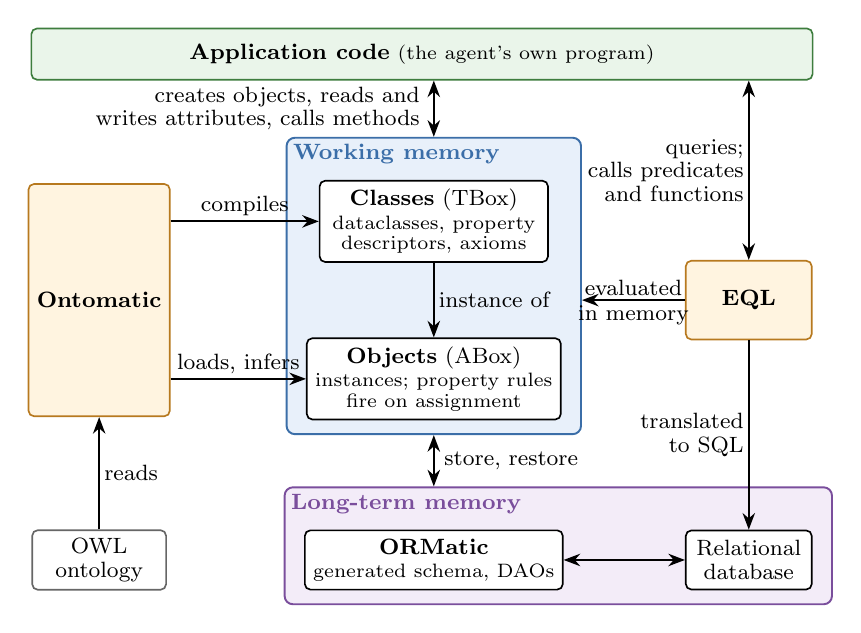
\begin{tikzpicture}[
  font=\footnotesize,
  >={Stealth[length=6pt,width=4.5pt]},
  box/.style={draw, rounded corners=2pt, align=center, inner sep=3pt, line width=0.6pt},
  inner/.style={box, fill=white, minimum width=2.9cm, minimum height=1.0cm},
  toolbox/.style={box, fill=tool, draw=toolline, minimum width=1.7cm, minimum height=0.7cm, font=\footnotesize\bfseries},
  lbl/.style={font=\footnotesize, align=left, inner sep=1.5pt},
  arr/.style={->, line width=0.7pt},
  group/.style={draw, rounded corners=3pt, line width=0.7pt, inner sep=5pt},
  title/.style={font=\footnotesize\bfseries, anchor=north west, inner sep=2.5pt},
]
% Grid: columns x=0 (Ontomatic), \xwm (working memory), \xeql (EQL, database);
% rows y=0 (classes), -2 (objects), \yltm (long-term memory).
\def\xwm{4.25}
\def\xeql{8.25}
\def\yltm{-4.3}

% --- Working memory -------------------------------------------------------
\node[inner] (classes) at (\xwm, 0) {\textbf{Classes} (TBox)\\[-1pt]
  {\scriptsize dataclasses, property}\\[-2pt]{\scriptsize descriptors, axioms}};
\node[inner] (objects) at (\xwm, -2.0) {\textbf{Objects} (ABox)\\[-1pt]
  {\scriptsize instances; property rules}\\[-2pt]{\scriptsize fire on assignment}};
\draw[arr] (classes) -- node[lbl, right] {instance of} (objects);

\path (classes.north) ++(0,0.36cm) coordinate (wmtop);
\begin{scope}[on background layer]
  \node[group, fill=wm, draw=wmline, fit=(classes)(objects)(wmtop), inner xsep=7pt] (wm) {};
\end{scope}
\node[title, text=wmline] at (wm.north west) {Working memory};

% --- Ontomatic (left): one tall box, so that both arrows are horizontal -----
\node[toolbox, minimum height=2.95cm, minimum width=1.6cm] (onto) at (0, -1.0) {Ontomatic};
\node[box, fill=white, draw=black!60, minimum width=1.7cm, minimum height=0.75cm]
  (owl) at (0, \yltm) {OWL\\[-1pt]ontology};
\draw[arr] (owl) -- node[lbl, right] {reads} (onto);
\draw[arr] (onto.east |- classes.west) -- node[lbl, above] {compiles} (classes.west);
\draw[arr] (onto.east |- objects.west) -- node[lbl, above] {loads, infers} (objects.west);

% --- EQL (right) ------------------------------------------------------------
\node[toolbox, minimum height=1.0cm, minimum width=1.6cm] (eql) at (\xeql, -1.0) {EQL};
\draw[arr] (eql.west) -- node[lbl, above, align=center] {evaluated}
  node[lbl, below, align=center] {in memory} (eql.west -| wm.east);

% --- Application code (top), spanning OWL ... EQL ---------------------------
\path (wm.north) ++(0,1.05cm) coordinate (apptop);
\node[box, fill=app, draw=appline, minimum height=0.65cm, inner sep=0pt,
      fit={(owl.west |- apptop) (eql.east |- apptop)}] (appbox) {};
\node at (appbox.center) {\textbf{Application code} {\scriptsize(the agent's own program)}};
\draw[arr, <->] (appbox.south -| wm.north) -- (wm.north);
\node[lbl, anchor=east, align=right] at ($(appbox.south -| wm.north)!0.5!(wm.north) + (-0.12,0)$)
  {creates objects, reads and\\[-1pt]writes attributes, calls methods};
\draw[arr, <->] (appbox.south -| eql.north) -- node[lbl, left, align=right] {queries;\\[-1pt]calls predicates\\[-1pt]and functions} (eql.north);

% --- Long-term memory (bottom) ---------------------------------------------
\node[box, fill=white, minimum width=2.9cm, minimum height=0.75cm] (ormatic)
  at (\xwm, \yltm) {\textbf{ORMatic}\\[-1pt]{\scriptsize generated schema, DAOs}};
\node[box, fill=white, minimum width=1.6cm, minimum height=0.75cm] (db)
  at (\xeql, \yltm) {Relational\\[-1pt]database};
\draw[arr, <->] (ormatic) -- (db);
\path (ormatic.north) ++(0,0.36cm) coordinate (ltmtop);
\begin{scope}[on background layer]
  \node[group, fill=ltm, draw=ltmline, fit=(ormatic)(db)(ltmtop), inner xsep=7pt] (ltm) {};
\end{scope}
\node[title, text=ltmline] at (ltm.north west) {Long-term memory};

\draw[arr, <->] (wm.south) -- node[lbl, right, xshift=2pt] {store, restore} (wm.south |- ltm.north);
\draw[arr] (eql.south) -- node[lbl, left, align=right] {translated\\[-1pt]to SQL} (eql.south |- db.north);

\end{tikzpicture}
\end{document}
